\subsection{Origen de los modelos neuronales}
%\begin{frame}{Origen de los modelos neuronales}
%	\begin{itemize}
%      	\item Ramón y Cajal
%      	\item McCulloch/Pitts
%      	\item Rosenblatt
%    \end{itemize}
    
%    \begin{figure}
%    \centering
%		    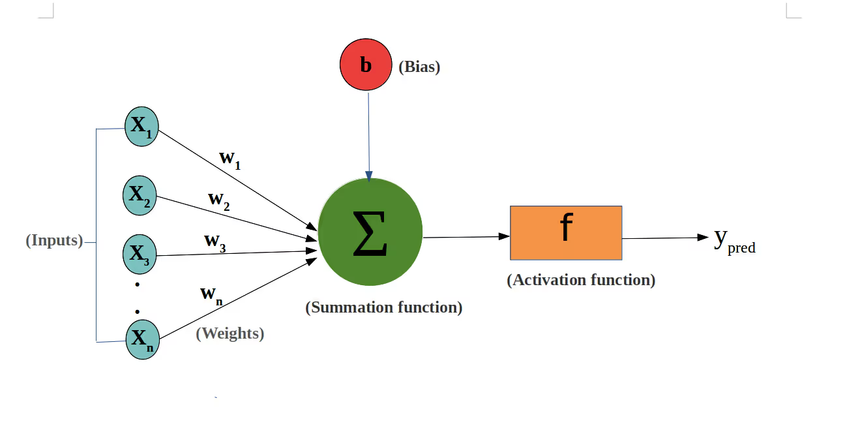
\includegraphics[width=\linewidth]{../Memoria/img/modelo/neuronaartificial.png}
%		    \caption{Esquema del funcionamiento de una neurona artificial.}
%		    \label{fig:neu-art}
%    \end{figure}
      
%    	\begin{figure}[H]
%	    \centering
%	    \hbox{
%	    \begin{minipage}[b]{0.25\textwidth}
%	    		\centering
%		    \includegraphics[width=\linewidth]{./img/RyC.png}
%		    \caption{Ramón y Cajal.}
%		    \label{fig:RyC}
%	    \end{minipage}
%	    
%	    \hspace{1cm}
%	        
%	    \begin{minipage}[b]{0.65\textwidth}
 %   			\centering
%		    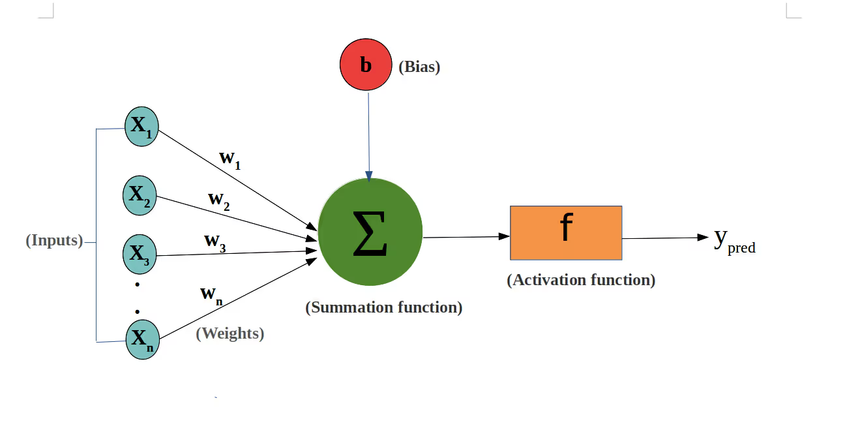
\includegraphics[width=\linewidth]{../Memoria/img/modelo/neuronaartificial.png}
%		    \caption{Esquema del funcionamiento de una neurona artificial 	%	\cite{tomorrow2023peso}.}
%		    \label{fig:neu-art}
%	    \end{minipage}	
%	    }
%	\end{figure}
	
%\end{frame}



\begin{frame}{Parámetros e hiperparámetros}

%\begin{itemize}
	
%	\item Los parámetros se ajustan a través del algoritmo de optimización, utilizando los cálculos de la función de pérdida durante la fase de entrenamiento de los modelos. Los parámetros de una red neuronal son:
%\begin{itemize}
%	\item Pesos.
%	\item Bias o sesgos.
%\end{itemize}
	 Los hiperparámetros son los responsables de controlar el comportamiento del proceso de entrenamiento. Algunos de los hiperparámetros más importantes son:
\begin{itemize}
	\item Tasa de aprendizaje (\textit{Learning rate}).
	\item Épocas (\textit{Epochs}).
	\item Tamaño de lote (\textit{Batch size}).
\end{itemize}

%\end{itemize}
    \begin{figure}
    \centering
		    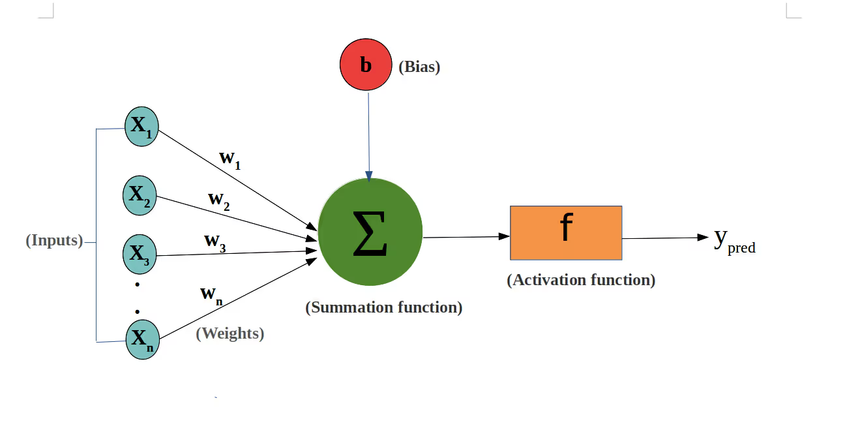
\includegraphics[width=0.75\linewidth]{../Memoria/img/modelo/neuronaartificial.png}
		    \caption{Esquema del funcionamiento de una neurona artificial.}
		    \label{fig:neu-art}
    \end{figure}

\end{frame}


\subsection{Clasificación con redes neuronales}
\begin{frame}{Matrices de confusión para el MCB}
\begin{itemize}
	\item \small Verdaderos positivos (VP).
    \item \small Falsos positivos (FP).
    \item \small Falsos negativos (FN).
    \item \small Verdaderos negativos (VN).
\end{itemize}

\begin{table}[H]
\centering
\begin{tabular}{|l|c|c|}
\hline
 & \textbf{Predicción Positiva} & \textbf{Predicción Negativa} \\ \hline
\textbf{Real Positivo} & VP & FN \\ \hline
\textbf{Real Negativo} & FP & VN \\ \hline
\end{tabular}
\caption{Matriz de confusión para modelos de clasificación binaria.}
\label{tab:confusion_matrix}
\end{table}

\scriptsize
\makebox[\textwidth][c]{%
  \begin{tabular}{c@{\hspace{1cm}}c@{\hspace{1cm}}c}
    $\displaystyle \text{Accuracy} = \frac{VP + VN}{VP + FP + VN + FN}$ &
    $\displaystyle \text{Precision} = \frac{VP}{VP + FP}$ &
    $\displaystyle \text{Recall} = \frac{VP}{VP + FN}$
  \end{tabular}
}






\end{frame}

\begin{frame}{Matriz de confusión para el MCM}
\begin{table}[H]
\centering
\resizebox{\textwidth}{!}{
\begin{tabular}{|>{\raggedright\arraybackslash}m{2.6cm}|*{9}{>{\centering\arraybackslash}m{2cm}|}}
\hline
  & \textbf{Predicción Clase 1} & \textbf{Predicción Clase 2} & \textbf{Predicción Clase 3} & \textbf{Predicción Clase 4} & \textbf{Predicción Clase 5} & \textbf{Predicción Clase 6} & \textbf{Predicción Clase 7} & \textbf{Predicción Clase 8} & \textbf{Predicción Clase 9} \\ \hline
\textbf{Real Clase 1} & \cellcolor{green!20}VP$_{1}$ & FP$_{12}$ & FP$_{13}$ & FP$_{14}$ & FP$_{15}$ & FP$_{16}$ & FP$_{17}$ & FP$_{18}$ & FP$_{19}$ \\ \hline
\textbf{Real Clase 2} & FP$_{21}$ & \cellcolor{green!20}VP$_{2}$ & FP$_{23}$ & FP$_{24}$ & FP$_{25}$ & FP$_{26}$ & FP$_{27}$ & FP$_{28}$ & FP$_{29}$ \\ \hline
\textbf{Real Clase 3} & FP$_{31}$ & FP$_{32}$ & \cellcolor{green!20}VP$_{3}$ & FP$_{34}$ & FP$_{35}$ & FP$_{36}$ & FP$_{37}$ & FP$_{38}$ & FP$_{39}$ \\ \hline
\textbf{Real Clase 4} & FP$_{41}$ & FP$_{42}$ & FP$_{43}$ & \cellcolor{green!20}VP$_{4}$ & FP$_{45}$ & FP$_{46}$ & FP$_{47}$ & FP$_{48}$ & FP$_{49}$ \\ \hline
\textbf{Real Clase 5} & FP$_{51}$ & FP$_{52}$ & FP$_{53}$ & FP$_{54}$ & \cellcolor{green!20}VP$_{5}$ & FP$_{56}$ & FP$_{57}$ & FP$_{58}$ & FP$_{59}$ \\ \hline
\textbf{Real Clase 6} & FP$_{61}$ & FP$_{62}$ & FP$_{63}$ & FP$_{64}$ & FP$_{65}$ & \cellcolor{green!20}VP$_{6}$ & FP$_{67}$ & FP$_{68}$ & FP$_{69}$ \\ \hline
\textbf{Real Clase 7} & FP$_{71}$ & FP$_{72}$ & FP$_{73}$ & FP$_{74}$ & FP$_{75}$ & FP$_{76}$ & \cellcolor{green!20}VP$_{7}$ & FP$_{78}$ & FP$_{79}$ \\ \hline
\textbf{Real Clase 8} & FP$_{81}$ & FP$_{82}$ & FP$_{83}$ & FP$_{84}$ & FP$_{85}$ & FP$_{86}$ & FP$_{87}$ & \cellcolor{green!20}VP$_{8}$ & FP$_{89}$ \\ \hline
\textbf{Real Clase 9} & FP$_{91}$ & FP$_{92}$ & FP$_{93}$ & FP$_{94}$ & FP$_{95}$ & FP$_{96}$ & FP$_{97}$ & FP$_{98}$ & \cellcolor{green!20}VP$_{9}$ \\ \hline
\end{tabular}
}
\caption{Matriz de confusión para los modelos de clasificación multiclase.}
\label{tab:confusion_matrix_9class}
\end{table}



\scriptsize
\begin{equation*}
F1_{\text{weighted}} = \sum_{c=1}^{C} \frac{N_c}{N} \cdot F1_c
\end{equation*}

Donde:
\begin{itemize}
    \item \( C \) es el número total de clases.
    \item \( N_c \) es el número de muestras de la clase \( c \).
    \item \( N \) es el número total de muestras.
    \item \( F1_c \) es la puntuación F1 de la clase \( c \), calculada como:
    

\[
    F1_c = 2 \cdot \frac{\text{Precision}_c \cdot \text{Recall}_c}{\text{Precision}_c + \text{Recall}_c}
    \]


\end{itemize}



\end{frame}


\begin{frame}{Perceptrón multicapa (MLP)}
	\begin{figure}
		\centering
	    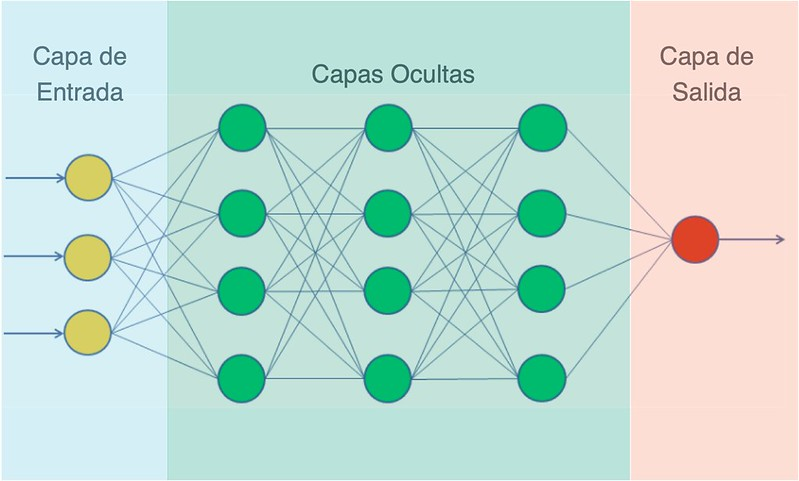
\includegraphics[width=\linewidth]{../Memoria/img/modelo/capas.png}
    		\caption{Esquema del perceptrón multicapa.}
	\end{figure}
\end{frame}




\begin{frame}{Patrón pizarra y Weights\&Biases}
	\begin{figure}
		\centering
	    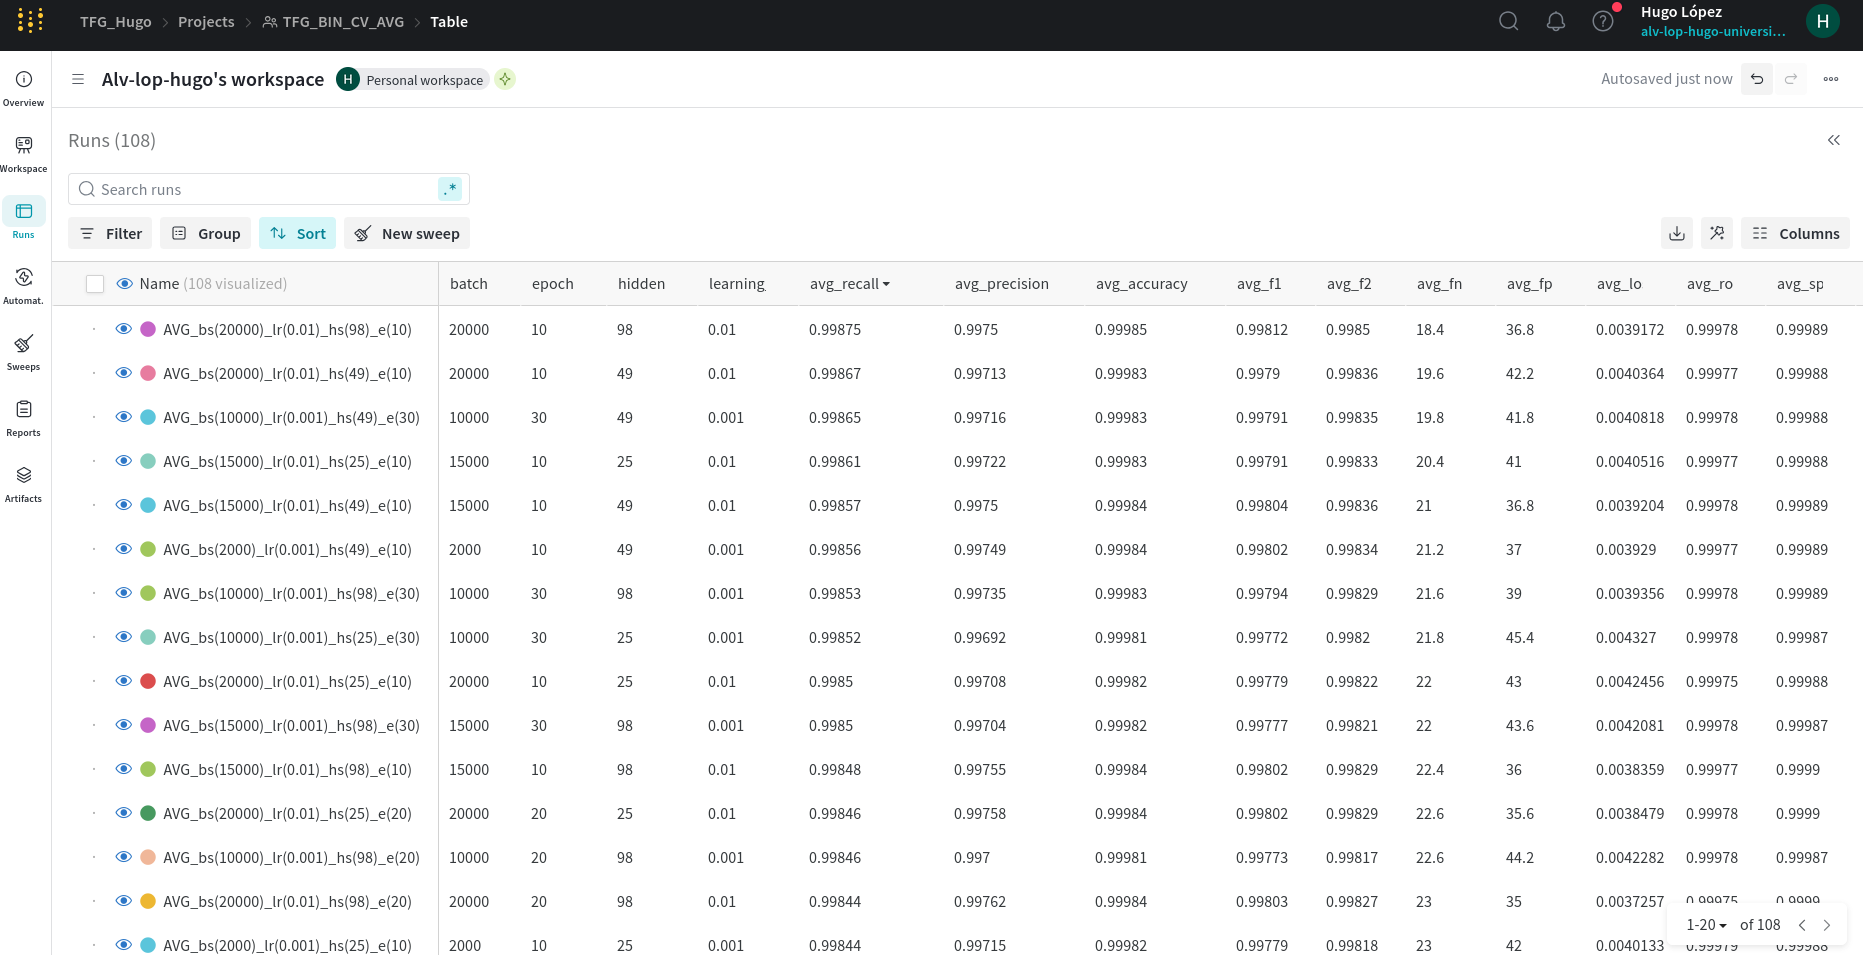
\includegraphics[width=\linewidth]{./img/wandb.png}
    		\caption{Ejemplo de utilización de Weights\&Biases como pizarra.}
	\end{figure}
\end{frame}




\subsection{Arquitecturas desarrolladas}
\begin{frame}{Arquitecturas desarrolladas para el MCB}
\begin{itemize}

	\item \textbf{MCB25}: Número de neuronas en la capa oculta igual a la mitad del número de atributos o entradas que recibe el modelo.
	\item \textbf{MCB49}: Número de neuronas en la capa oculta igual al mismo número de atributos o entradas que recibe el modelo.
	\item \textbf{MCB98}: Número de neuronas en la capa oculta igual al doble del número de atributos o entradas que recibe el modelo. 

\end{itemize}

    	\begin{figure}[H]
	    \centering
	    \hbox{
	    \begin{minipage}{0.3\textwidth}
	    		\centering
		    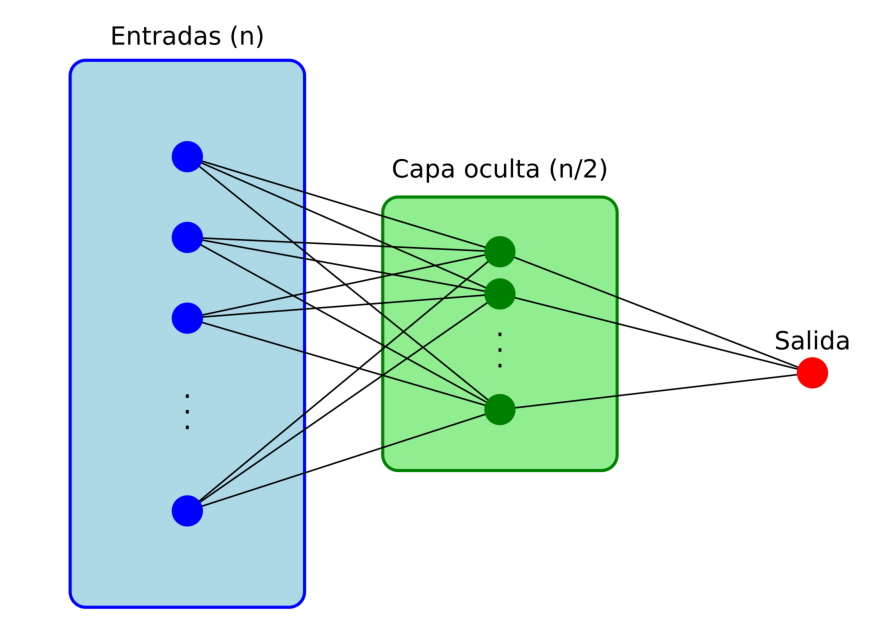
\includegraphics[width=\linewidth]{../Memoria/img/modelo/arquitecturas/arqnmediosBIN.pdf}
    \caption{MCB25.}
	    \end{minipage}
	    
	    \hspace{.5cm}
	        
	    \begin{minipage}{0.3\textwidth}
    			\centering
		    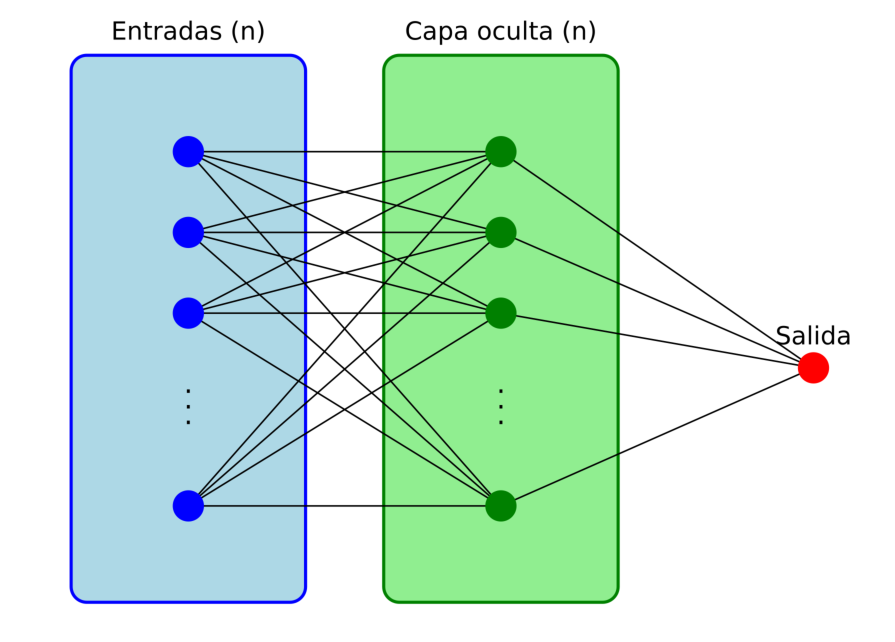
\includegraphics[width=\linewidth]{../Memoria/img/modelo/arquitecturas/arqnBIN.pdf}
		    \caption{MCB49.}
	    \end{minipage}	
	    \hspace{.5cm}
	        
	    \begin{minipage}{0.3\textwidth}
    			\centering
		    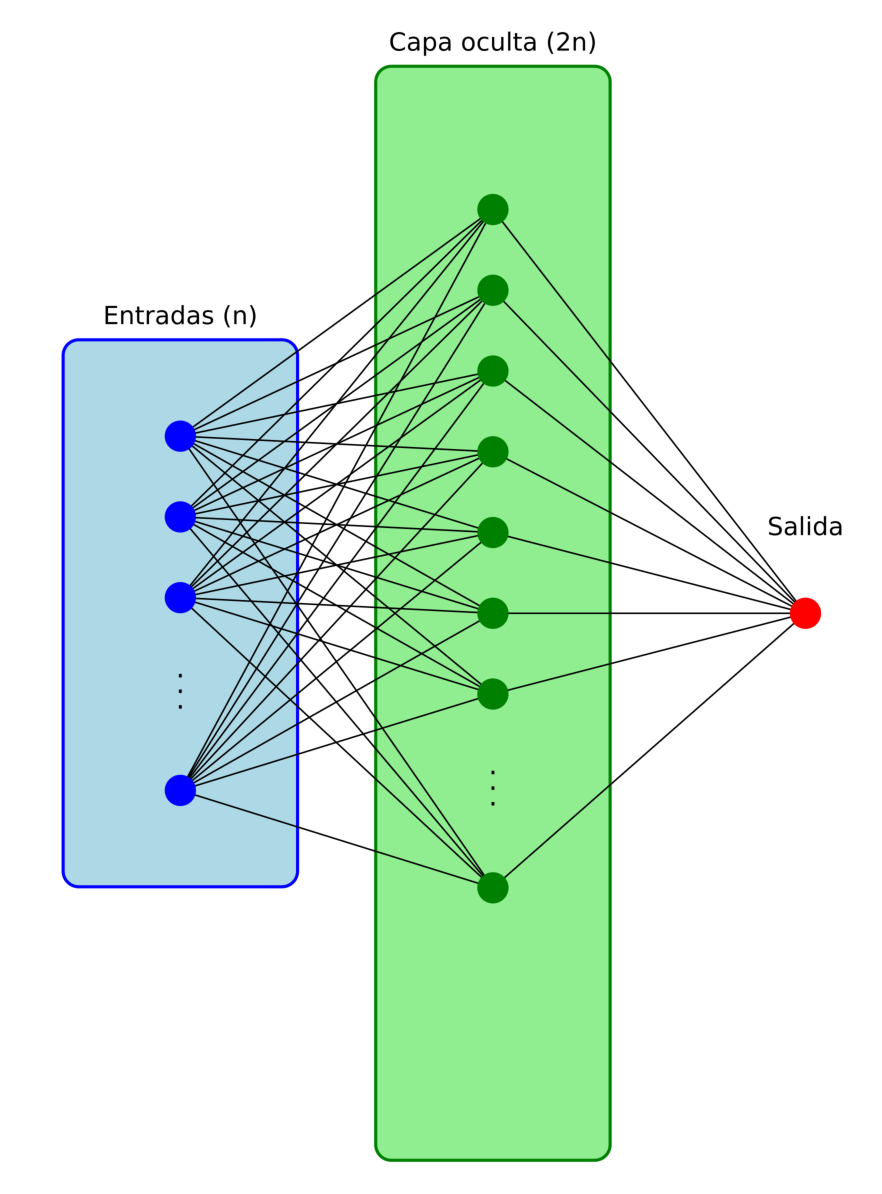
\includegraphics[width=\linewidth]{../Memoria/img/modelo/arquitecturas/arqnnBIN.pdf}
		    \caption{MCB98.}
	    \end{minipage}
	    }
	\end{figure}
	
\end{frame}


\begin{frame}{Arquitecturas desarrolladas para el MCM}
\begin{itemize}


	\item \textbf{MCM25}: Número de neuronas en la capa oculta igual a la mitad del número de atributos o entradas que recibe el modelo.
	\item \textbf{MCM49}: Número de neuronas en la capa oculta igual al mismo número de atributos o entradas que recibe el modelo.
	\item \textbf{MCM98}: Número de neuronas en la capa oculta igual al doble del número de atributos o entradas que recibe el modelo.
\end{itemize}
    	\begin{figure}[H]
	    \centering
	    \hbox{
	    \begin{minipage}{0.3\textwidth}
	    		\centering
		    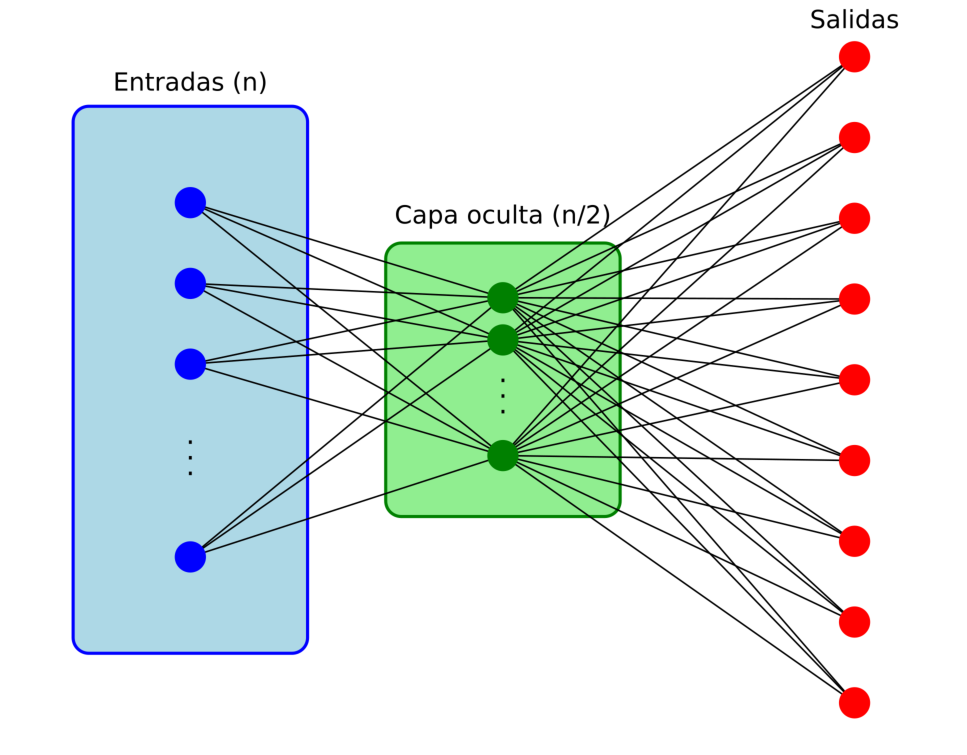
\includegraphics[width=\linewidth]{../Memoria/img/modelo/arquitecturas/arqnmediosMUL.pdf}
    \caption{MCM25.}
	    \end{minipage}
	    
	    \hspace{.5cm}
	        
	    \begin{minipage}{0.3\textwidth}
    			\centering
		    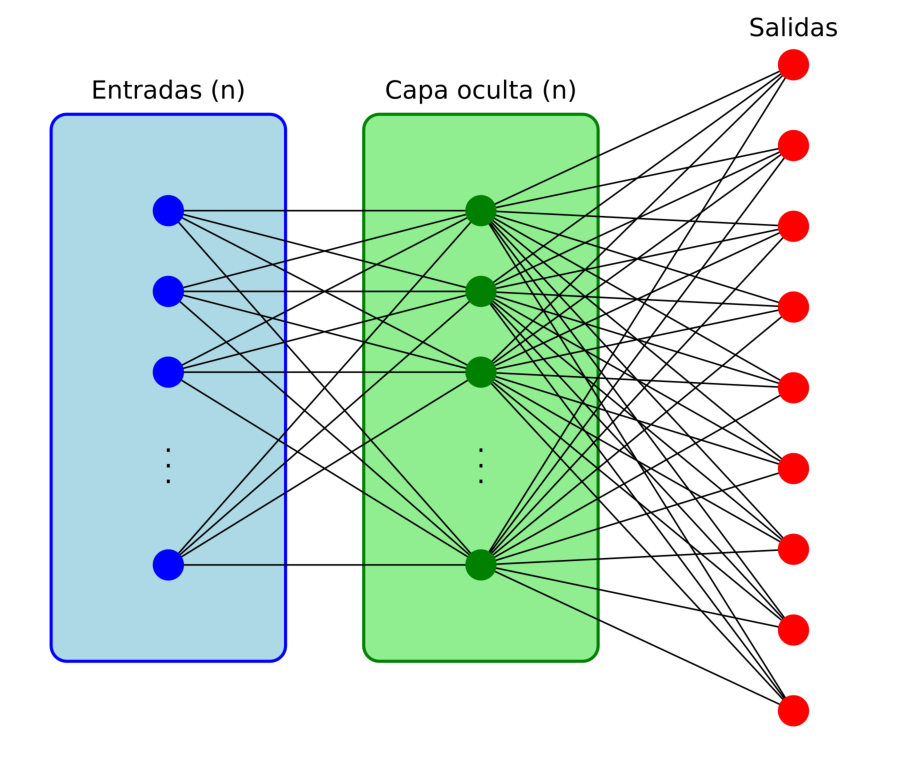
\includegraphics[width=\linewidth]{../Memoria/img/modelo/arquitecturas/arqnMUL.pdf}
		    \caption{MCM49.}
	    \end{minipage}	
	    \hspace{.5cm}
	        
	    \begin{minipage}{0.3\textwidth}
    			\centering
		    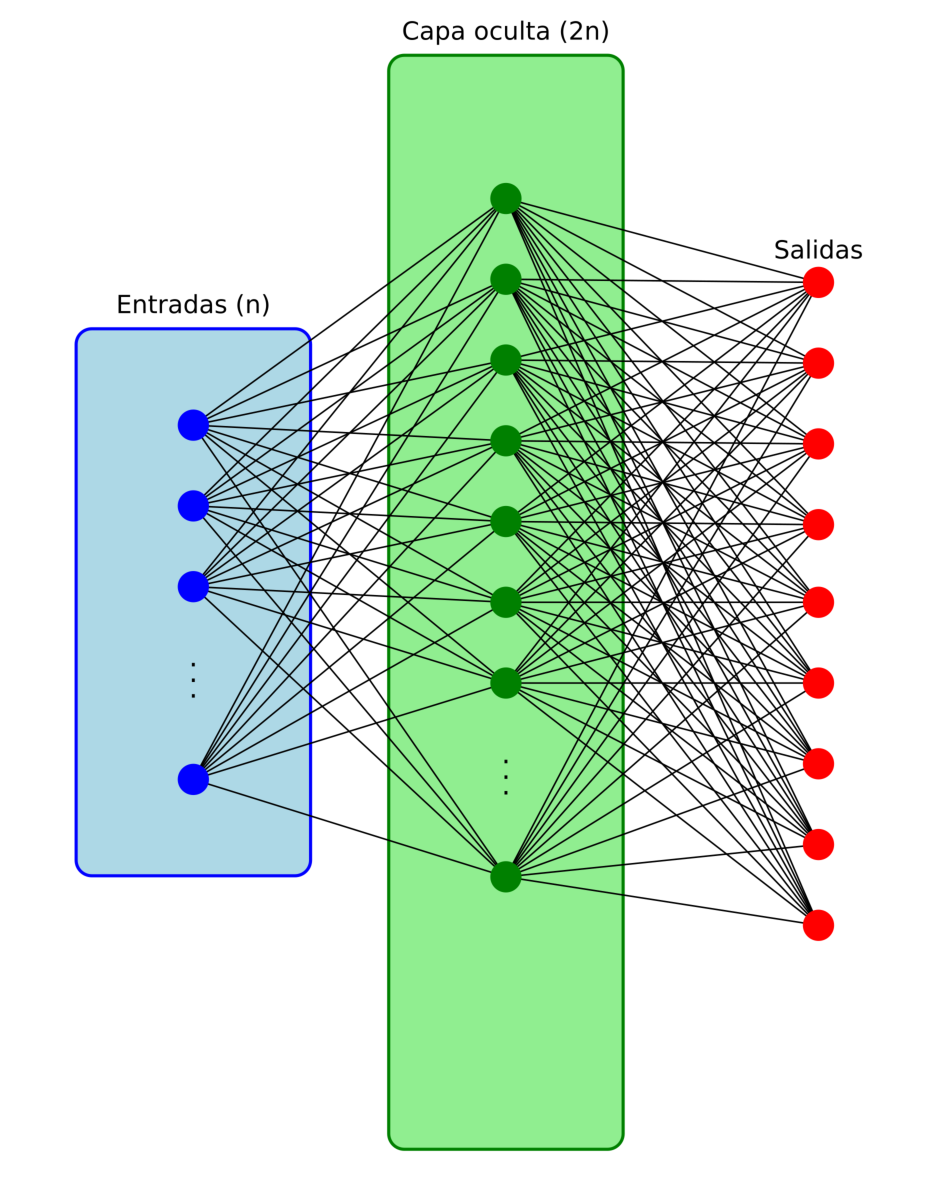
\includegraphics[width=\linewidth]{../Memoria/img/modelo/arquitecturas/arqnnMUL.pdf}
		    \caption{MCM98.}
	    \end{minipage}
	    }
	\end{figure}
	
\end{frame}


\subsection{Implementación de los modelos}
\begin{frame}{Validación cruzada}

	\begin{figure}
		\centering
	    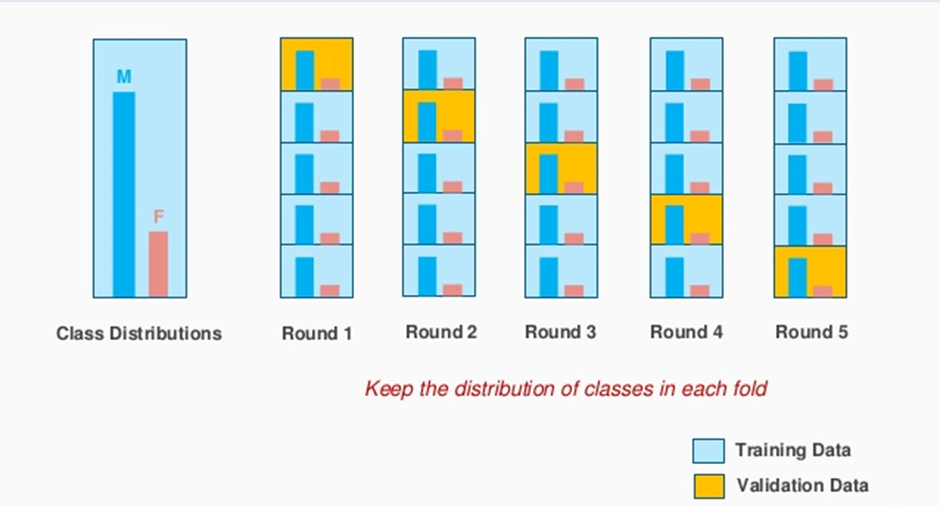
\includegraphics[width=\linewidth]{./img/stratifiedkfolds.png}
    		\caption{Esquema de la validación cruzada (\textit{Stratificate k-fold} (5 \textit{folds}).}
	\end{figure}

\end{frame}

\begin{frame}{Implementación del MCB}
	\begin{itemize}
		\item \textbf{Función de pérdida}: \texttt{BCEWithLogistLoss}
		\item \textbf{Algoritmo de optimización}: \texttt{AdamW}
	\end{itemize}
	
%	\begin{figure}[H]
%	    \centering
%	    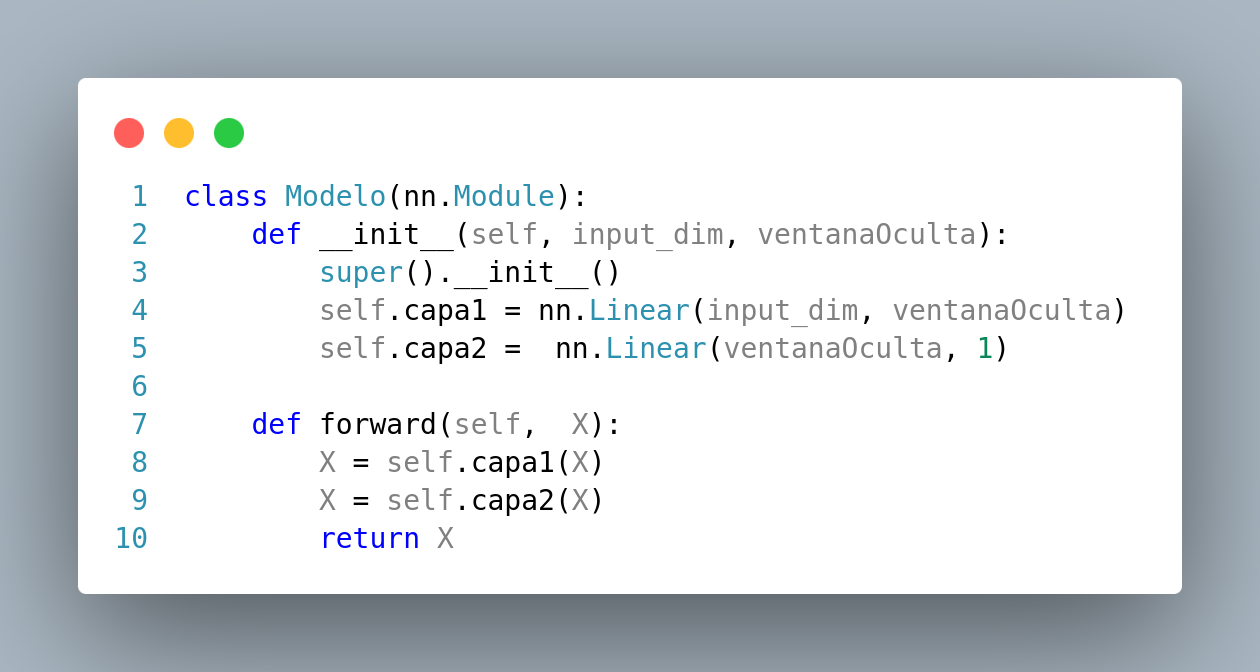
\includegraphics[width=0.6\textwidth]{../Memoria/img/modelo/codigo/modeloBIN.png}
%	    	\caption{Definición de la clase del modelo de clasificación binaria.}
%   		\label{fig:modBIN}
%	\end{figure}
	
	\begin{table}[H]
		\centering 
		\resizebox{0.6\textwidth}{!}{
		\begin{tabular}{|c|c|}
		\hline
		\textbf{Hiperparámetro} & \textbf{Posibles valores} \\ \hline
		\textit{Batch size} & [2000, 10000, 15000, 20000] \\ \hline
		\textit{Learning rate} & [$10^{-2}$, $10^{-3}$, $10^{-4}$] \\ \hline
		Épocas & [10, 20, 30] \\ \hline
		\end{tabular}
		}
		\caption{Valores de los hiperparámetros utilizados en los experimentos del modelo de clasificación binaria.}
		\label{tab:hiperBIN}
	\end{table}
\end{frame}

\begin{frame}{Implementación del MCM}
	\begin{itemize}
		\item \textbf{Función de pérdida}: \texttt{CrossEntropyLoss}
		\item \textbf{Algoritmo de optimización}: \texttt{AdamW}
	\end{itemize}
	
%	\begin{figure}[H]
%	    \centering
%	    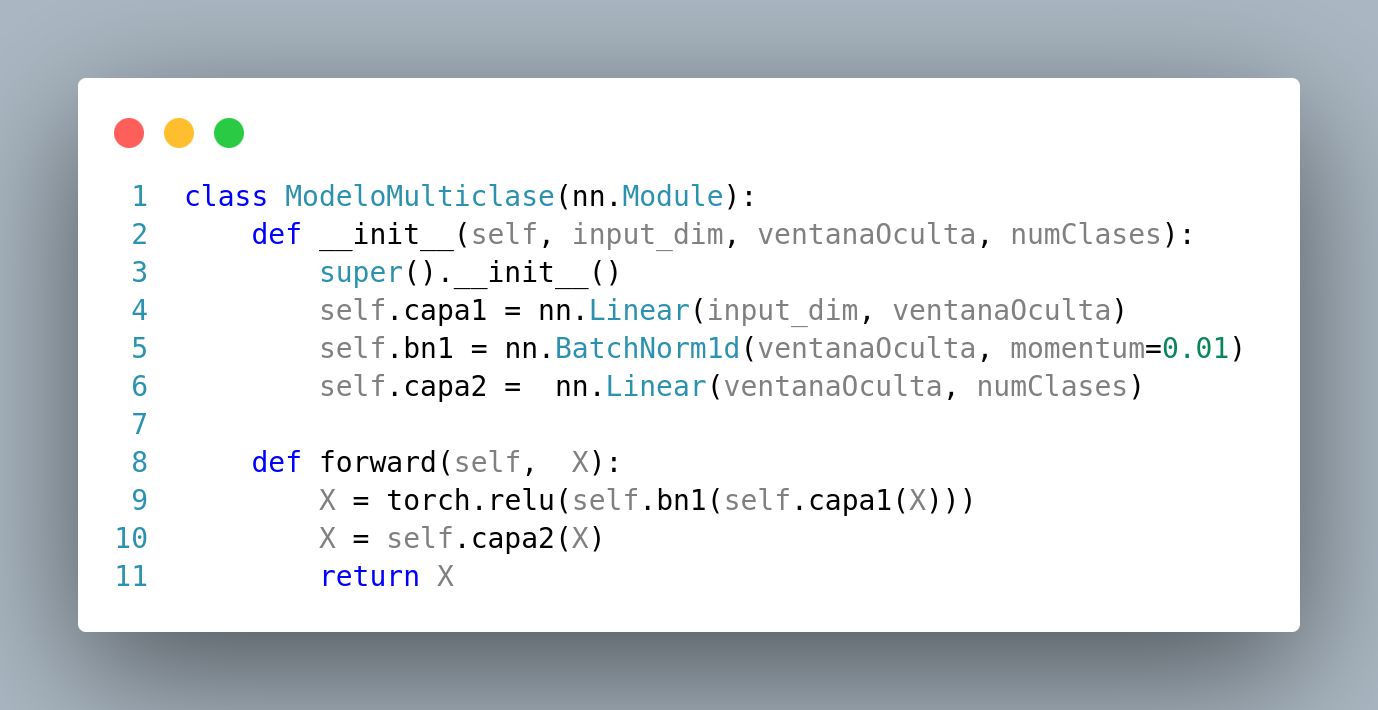
\includegraphics[width=0.6\textwidth]{../Memoria/img/modelo/codigo/modeloMUL.png}
%	    	\caption{Definición de la clase del modelo de clasificación multiclase.}
%    		\label{fig:modBIN}
%	\end{figure}
	
	\begin{table}[H]
		\centering 
		\resizebox{0.6\textwidth}{!}{
		\begin{tabular}{|c|c|}
		\hline
		\textbf{Hiperparámetro} & \textbf{Posibles valores} \\ \hline
		\textit{Batch size} & [32, 64, 128, 256, 512] \\ \hline
		\textit{Learning rate} & [$10^{-2}$, $10^{-3}$, $10^{-4}$, $10^{-5}$] \\ \hline
		Épocas & [30, 50, 80, 100] \\ \hline
		\end{tabular}
		}
		\caption{Valores de los hiperparámetros utilizados en los experimentos del modelo de clasificación multiclase.}
		\label{tab:hiperBIN}
	\end{table}
\end{frame}



\subsection{Selección de las configuraciones de los modelos}

\begin{frame}{Selección de los mejores MCB}
Los mejores resultados del MCB los obtuvo la arquitectura con el doble de neuronas en su capa oculta que atributos de entrada tiene el modelo.
\begin{columns}[b]
\begin{column}{0.7\textwidth}
\begin{table}[H]
		\resizebox{1\textwidth}{!}{
\begin{tabular}{|>{\columncolor[HTML]{E0FFFF}}l|c|c|c|c|c|}
\hline
Posicion\_EXP & 1º-MCB98 & 2º-MCB98 & 3º-MCB98 & 4º-MCB98 & 5º-MCB98 \\
\hline
\cellcolor[HTML]{E0FFFF}batch\_size & \cellcolor[HTML]{66ffa8}20000 & \cellcolor[HTML]{66ffa8}10000 & \cellcolor[HTML]{66ffa8}15000 & \cellcolor[HTML]{66ffa8}15000 & \cellcolor[HTML]{66ffa8}10000 \\
\cellcolor[HTML]{E0FFFF}epochs & \cellcolor[HTML]{b1bafb}10 & \cellcolor[HTML]{b1bafb}30 & \cellcolor[HTML]{b1bafb}30 & \cellcolor[HTML]{b1bafb}10 & \cellcolor[HTML]{b1bafb}20 \\
\cellcolor[HTML]{E0FFFF}learning\_rate & \cellcolor[HTML]{f99595}$10^{-2}$ & \cellcolor[HTML]{f99595}$10^{-3}$ & \cellcolor[HTML]{f99595}$10^{-3}$ & \cellcolor[HTML]{f99595}$10^{-2}$ & \cellcolor[HTML]{f99595}$10^{-3}$ \\
\cellcolor[HTML]{E0FFFF}avg\_f1 & 0.998124 & 0.997941 & 0.997771 & 0.998015 & 0.997730 \\
\cellcolor[HTML]{E0FFFF}avg\_fn & 18.4 & 21.6 & 22 & 22.4 & 22.6 \\
\cellcolor[HTML]{E0FFFF}avg\_fp & 36.8 & 39 & 43.6 & 36 & 44.2 \\
\cellcolor[HTML]{E0FFFF}avg\_precision & 0.997501 & 0.997351 & 0.997039 & 0.997554 & 0.996999 \\
\cellcolor[HTML]{E0FFFF}avg\_recall & 0.998749 & 0.998531 & 0.998504 & 0.998477 & 0.998463 \\
\cellcolor[HTML]{E0FFFF}avg\_roc\_auc & 0.999781 & 0.999777 & 0.999776 & 0.999773 & 0.999777 \\
\cellcolor[HTML]{E0FFFF}avg\_tn & 344127.4 & 344125.2 & 344120.6 & 344128.2 & 344120 \\
\cellcolor[HTML]{E0FFFF}avg\_tp & 14686.2 & 14683 & 14682.6 & 14682.2 & 14682 \\
\hline
\end{tabular}
}
    \caption{Mejores cinco configuraciones para el MCB98.}
    \label{fig:BINhs98}
\end{table}
\end{column}

\begin{column}{0.3\textwidth}
\begin{figure}[H]
    \centering
    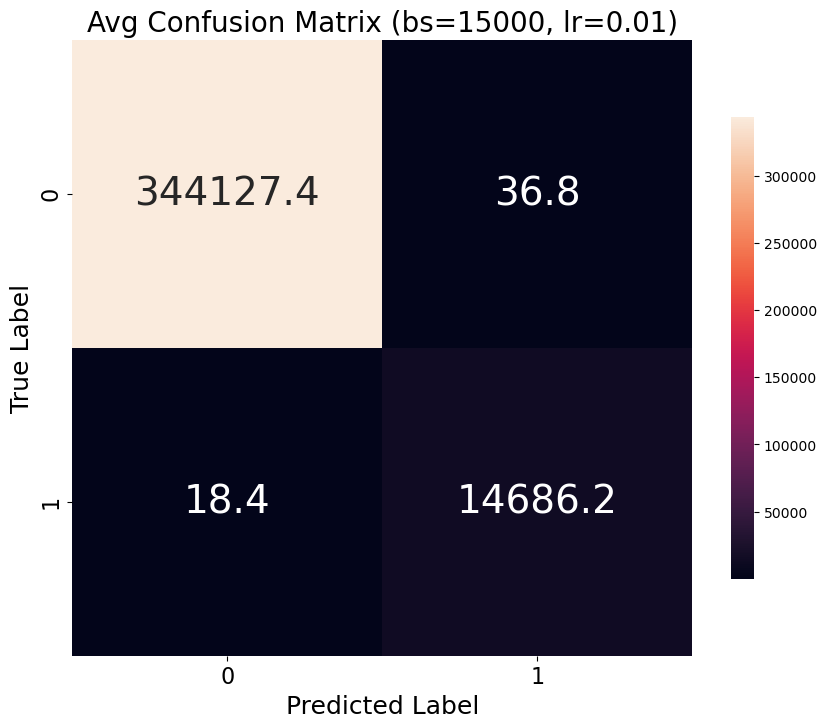
\includegraphics[width=1\textwidth]{../Memoria/img/modelo/matrices_confusion/MC_ENT_MCB98.png}
    \caption{Matriz de confusión 1º MCB98.}
    \label{fig:MC_ENT_MCB98}
\end{figure}

\end{column}
\end{columns}
\end{frame}


\begin{frame}{Mejores 5 configuraciones del MCB}
En este modelo no se observa que la arquitectura influya especialmente en los resultados obtenidos.
\begin{figure}[H]
    \centering
    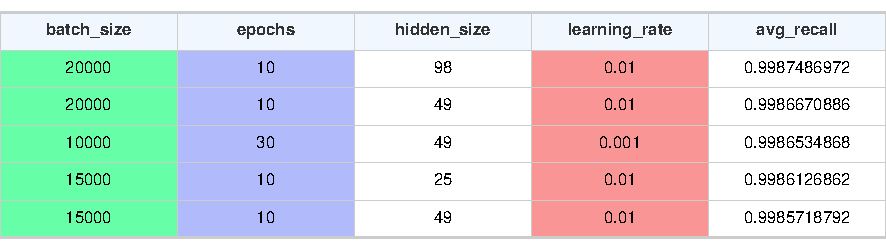
\includegraphics[width=0.85\textwidth]{../Memoria/img/modelo/resultados/BINtop5.pdf}
    \caption{Mejores cinco configuraciones de hiperparámetros del modelo de clasificación binaria.}
    \label{fig:BINtop5}
\end{figure}

\end{frame}




\begin{frame}{Selección de los mejores MCM}
Al igual que en el MCB, los mejores resultados del MCM se han obtenido en la arquitectura con el doble de neuronas en su capa oculta que atributos de entrada tiene el modelo.
\begin{columns}[b]
\begin{column}{0.6\textwidth}
\begin{table}[H]
		\resizebox{1\textwidth}{!}{
\begin{tabular}{|>{\columncolor[HTML]{E0FFFF}}l|c|c|c|c|c|}
\hline
Posicion\_EXP & 1º-MCM98 & 2º-MCM98 & 3º-MCM98 & 4º-MCM98 & 5º-MCM98 \\
\hline
\cellcolor[HTML]{E0FFFF}batch\_size & \cellcolor[HTML]{66ffa8}256 & \cellcolor[HTML]{66ffa8}256 & \cellcolor[HTML]{66ffa8}512 & \cellcolor[HTML]{66ffa8}64 & \cellcolor[HTML]{66ffa8}256 \\
\cellcolor[HTML]{E0FFFF}epochs & \cellcolor[HTML]{b1bafb}100 & \cellcolor[HTML]{b1bafb}80 & \cellcolor[HTML]{b1bafb}100 & \cellcolor[HTML]{b1bafb}80 & \cellcolor[HTML]{b1bafb}50 \\
\cellcolor[HTML]{E0FFFF}learning\_rate & \cellcolor[HTML]{f99595}$10^{-3}$ & \cellcolor[HTML]{f99595}$10^{-3}$ & \cellcolor[HTML]{f99595}$10^{-2}$ & \cellcolor[HTML]{f99595}$10^{-3}$ & \cellcolor[HTML]{f99595}$10^{-3}$ \\
\cellcolor[HTML]{E0FFFF}avg\_accuracy & 0.569414 & 0.556057 & 0.556915 & 0.556969 & 0.562083 \\
\cellcolor[HTML]{E0FFFF}avg\_f1\_macro & 0.413180 & 0.406773 & 0.388808 & 0.398720 & 0.397308 \\
\cellcolor[HTML]{E0FFFF}avg\_f1\_weighted & 0.583123 & 0.577553 & 0.574200 & 0.571020 & 0.569831 \\
\cellcolor[HTML]{E0FFFF}avg\_precision\_macro & 0.394898 & 0.385322 & 0.372836 & 0.377543 & 0.387029 \\
\cellcolor[HTML]{E0FFFF}avg\_precision\_weighted & 0.681971 & 0.675326 & 0.674534 & 0.669836 & 0.669688 \\
\cellcolor[HTML]{E0FFFF}avg\_recall\_macro & 0.577069 & 0.564962 & 0.573083 & 0.566046 & 0.550391 \\
\cellcolor[HTML]{E0FFFF}avg\_recall\_weighted & 0.569414 & 0.556057 & 0.556915 & 0.556969 & 0.562083 \\
\cellcolor[HTML]{E0FFFF}avg\_roc\_auc\_ovo & 0.813320 & 0.806782 & 0.809286 & 0.812789 & 0.800316 \\
\cellcolor[HTML]{E0FFFF}avg\_roc\_auc\_ovr & 0.788041 & 0.784984 & 0.781135 & 0.782758 & 0.777422 \\
\hline
\end{tabular}
}
    \caption{Mejores cinco configuraciones para el MCM98.}
    \label{fig:MULhs98}
\end{table}
\end{column}

\begin{column}{0.55\textwidth}
\begin{figure}[H]
    \centering
    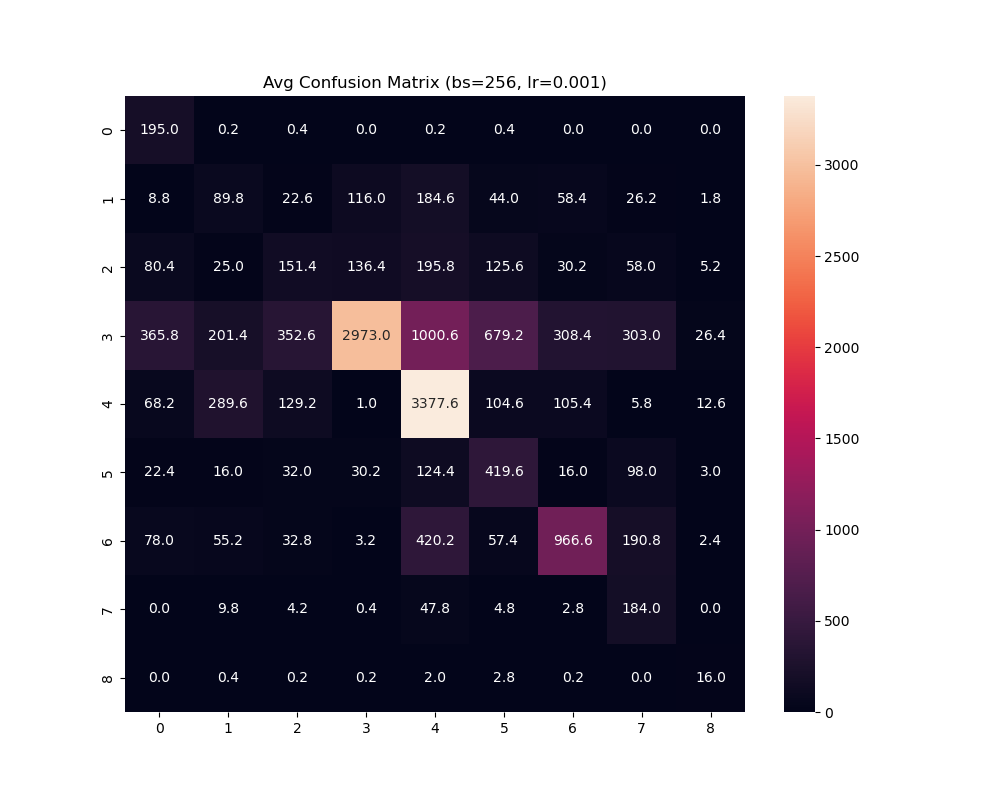
\includegraphics[width=1\textwidth]{../Memoria/img/modelo/matrices_confusion/MC_ENT_MCM98.png}
    \caption{Matriz de confusión 1º MCM98.}
    \label{fig:MC_ENT_MCM98}
\end{figure}

\end{column}
\end{columns}
\end{frame}


\begin{frame}{Mejores 10 configuraciones del MCM}
En el caso del MCM, la arquitectura MCM98 ha obtenido en la fase de entrenamiento unos resultados muy superiores a las otras dos arquitecturas desarrolladas.
\begin{figure}[H]
    \centering
    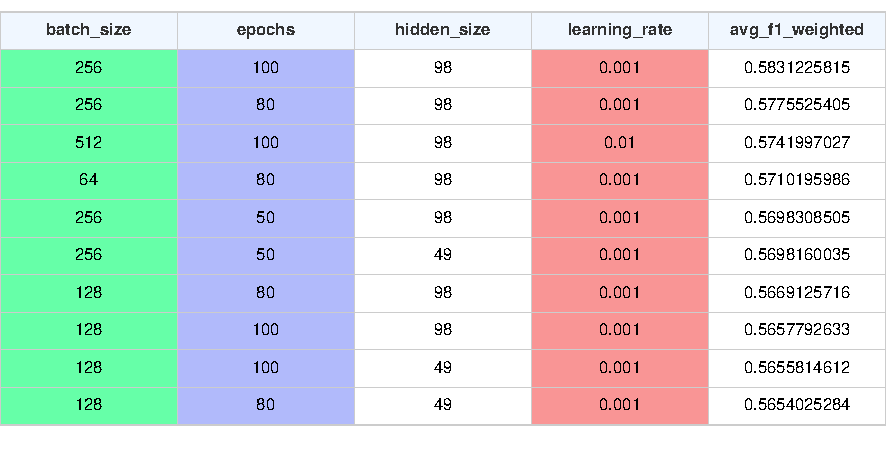
\includegraphics[width=1\textwidth]{../Memoria/img/modelo/resultados/MULtop10.pdf}
    \caption{Mejores diez configuraciones de hiperparámetros del modelo de clasificación multiclase.}
    \label{fig:BINtop5}
\end{figure}

\end{frame}




























